% Created by tikzDevice version 0.6.2-92-0ad2792 on 2013-12-01 00:58:43
% !TEX encoding = UTF-8 Unicode
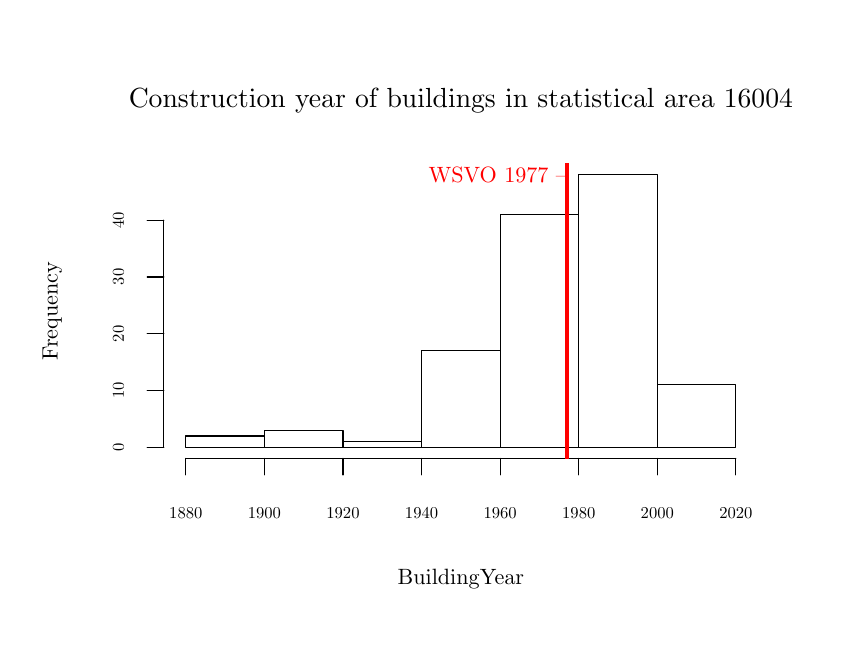
\begin{tikzpicture}[x=1pt,y=1pt]
\definecolor[named]{fillColor}{rgb}{1.00,1.00,1.00}
\path[use as bounding box,fill=fillColor,fill opacity=0.00] (0,0) rectangle (289.08,216.81);
\begin{scope}
\path[clip] (  0.00,  0.00) rectangle (289.08,216.81);
\definecolor[named]{drawColor}{rgb}{0.00,0.00,0.00}

\node[text=drawColor,anchor=base,inner sep=0pt, outer sep=0pt, scale=  1.0] at
(156.54,188.07) {Construction year of buildings in statistical area 16004};

\node[text=drawColor,anchor=base,inner sep=0pt, outer sep=0pt, scale=  0.8] at (156.54, 15.60) {BuildingYear};

\node[text=drawColor,rotate= 90.00,anchor=base,inner sep=0pt, outer sep=0pt,
scale=  0.8] at ( 10.80,114.41) {Frequency};
\end{scope}
\begin{scope}
\path[clip] (  0.00,  0.00) rectangle (289.08,216.81);
\definecolor[named]{drawColor}{rgb}{0.00,0.00,0.00}

\path[draw=drawColor,line width= 0.4pt,line join=round,line cap=round] ( 57.15, 61.20) -- (255.93, 61.20);

\path[draw=drawColor,line width= 0.4pt,line join=round,line cap=round] ( 57.15, 61.20) -- ( 57.15, 55.20);

\path[draw=drawColor,line width= 0.4pt,line join=round,line cap=round] ( 85.55, 61.20) -- ( 85.55, 55.20);

\path[draw=drawColor,line width= 0.4pt,line join=round,line cap=round] (113.94, 61.20) -- (113.94, 55.20);

\path[draw=drawColor,line width= 0.4pt,line join=round,line cap=round] (142.34, 61.20) -- (142.34, 55.20);

\path[draw=drawColor,line width= 0.4pt,line join=round,line cap=round] (170.74, 61.20) -- (170.74, 55.20);

\path[draw=drawColor,line width= 0.4pt,line join=round,line cap=round] (199.14, 61.20) -- (199.14, 55.20);

\path[draw=drawColor,line width= 0.4pt,line join=round,line cap=round] (227.53, 61.20) -- (227.53, 55.20);

\path[draw=drawColor,line width= 0.4pt,line join=round,line cap=round] (255.93, 61.20) -- (255.93, 55.20);

\node[text=drawColor,anchor=base,inner sep=0pt, outer sep=0pt, scale=  0.6] at ( 57.15, 39.60) {1880};

\node[text=drawColor,anchor=base,inner sep=0pt, outer sep=0pt, scale=  0.6] at ( 85.55, 39.60) {1900};

\node[text=drawColor,anchor=base,inner sep=0pt, outer sep=0pt, scale=  0.6] at (113.94, 39.60) {1920};

\node[text=drawColor,anchor=base,inner sep=0pt, outer sep=0pt, scale=  0.6] at (142.34, 39.60) {1940};

\node[text=drawColor,anchor=base,inner sep=0pt, outer sep=0pt, scale=  0.6] at (170.74, 39.60) {1960};

\node[text=drawColor,anchor=base,inner sep=0pt, outer sep=0pt, scale=  0.6] at (199.14, 39.60) {1980};

\node[text=drawColor,anchor=base,inner sep=0pt, outer sep=0pt, scale=  0.6] at (227.53, 39.60) {2000};

\node[text=drawColor,anchor=base,inner sep=0pt, outer sep=0pt, scale=  0.6] at (255.93, 39.60) {2020};

\path[draw=drawColor,line width= 0.4pt,line join=round,line cap=round] ( 49.20, 65.14) -- ( 49.20,147.25);

\path[draw=drawColor,line width= 0.4pt,line join=round,line cap=round] ( 49.20, 65.14) -- ( 43.20, 65.14);

\path[draw=drawColor,line width= 0.4pt,line join=round,line cap=round] ( 49.20, 85.67) -- ( 43.20, 85.67);

\path[draw=drawColor,line width= 0.4pt,line join=round,line cap=round] ( 49.20,106.19) -- ( 43.20,106.19);

\path[draw=drawColor,line width= 0.4pt,line join=round,line cap=round] ( 49.20,126.72) -- ( 43.20,126.72);

\path[draw=drawColor,line width= 0.4pt,line join=round,line cap=round] ( 49.20,147.25) -- ( 43.20,147.25);

\node[text=drawColor,rotate= 90.00,anchor=base,inner sep=0pt, outer sep=0pt,
scale=  0.6] at ( 34.80, 65.14) {0};

\node[text=drawColor,rotate= 90.00,anchor=base,inner sep=0pt, outer sep=0pt,
scale=  0.6] at ( 34.80, 85.67) {10};

\node[text=drawColor,rotate= 90.00,anchor=base,inner sep=0pt, outer sep=0pt, scale=  0.6] at ( 34.80,106.19) {20};

\node[text=drawColor,rotate= 90.00,anchor=base,inner sep=0pt, outer sep=0pt, scale=  0.6] at ( 34.80,126.72) {30};

\node[text=drawColor,rotate= 90.00,anchor=base,inner sep=0pt, outer sep=0pt, scale=  0.6] at ( 34.80,147.25) {40};
\end{scope}
\begin{scope}
\path[clip] ( 49.20, 61.20) rectangle (263.88,167.61);
\definecolor[named]{drawColor}{rgb}{0.00,0.00,0.00}

\path[draw=drawColor,line width= 0.4pt,line join=round,line cap=round] ( 57.15, 65.14) rectangle ( 85.55, 69.25);

\path[draw=drawColor,line width= 0.4pt,line join=round,line cap=round] ( 85.55, 65.14) rectangle (113.94, 71.30);

\path[draw=drawColor,line width= 0.4pt,line join=round,line cap=round] (113.94, 65.14) rectangle (142.34, 67.19);

\path[draw=drawColor,line width= 0.4pt,line join=round,line cap=round] (142.34, 65.14) rectangle (170.74,100.04);

\path[draw=drawColor,line width= 0.4pt,line join=round,line cap=round] (170.74, 65.14) rectangle (199.14,149.30);

\path[draw=drawColor,line width= 0.4pt,line join=round,line cap=round] (199.14, 65.14) rectangle (227.53,163.67);

\path[draw=drawColor,line width= 0.4pt,line join=round,line cap=round] (227.53, 65.14) rectangle (255.93, 87.72);
\definecolor[named]{drawColor}{rgb}{1.00,0.00,0.00}

\path[draw=drawColor,line width= 1.6pt,line join=round,line cap=round] (194.88, 61.20) -- (194.88,167.61);

\node[text=drawColor,anchor=base east,inner sep=0pt, outer sep=0pt, scale=  0.8] at (194.88,160.89) {WSVO 1977 --};
\end{scope}
\end{tikzpicture}
